
\chapter{Model Overview}
\label{ch:model-overview}

\section{Environment}

The computational model describes the environment as a set of connected nodes, objects that implement the \emph{Node} interface. These nodes can be connected as the user wish, creating one, two or three dimensional environments, agents are capable to navigate from nodes to their neighbours, read communication stimuli deposited in the nodes by another agents and alter the environment themselves by depositing communication stimuli if they require.

As we will see the \emph{Node} interface does not formalises how the nodes are connected, so users have the freedom to create the environments that suit their experiments. The standard implementation uses 2 dimensional grids, with each node connected to a maximum of 4 neighbours, one in each possible direction listed in the enumeration \emph{Direction}.

\subsection{Nodes}

The fundamental entity to represent the environment the \emph{Node} interface. A node can be seen as an infinitesimal piece of the environment. By linking nodes together it is possible to create complex network of objects that will describe the space where agents can navigate.

The \emph{Node} interface does not specify how these connections need to be made and how many neighbours each node has. This gives a great degree of freedom to users, for example it is ease to declare different types of nodes, that can describe different types of environment. For example, the \emph{BasicNode} class is used to describe two dimensional environments, as we will see later on. A three dimensional environment could be easily described as well though, by implementing the \emph{Node} interface with 6 neighbours, one in each direction - north, south, east, west, above and bellow, agents would be able to navigate through nodes in three different axis.

(((add and describe methods for neighbours)))

Each node has an unique string that is used to identify them. The method \emph{getId()} returns this string, which should be unique. Note that the \emph{Node} interface does not have any instrument to guarantee that nodes have unique identifiers, it is up to the users of the interface to guarantee that nodes do not have duplicated identifiers. 

Nodes also have a list of agents (see section \ref{sec:agents}), this is the list of agents that are currently in the node. The node interface provides the necessary methods to operate upon the agents, these are:

\begin{itemize}
  \item void addAgent(Agent): Verify if the agent can be added to the node, if yes, adds the agent to the node, if not ignores..
  \item List<Agent> getAgents(): Return the list of agents currently in the node
  \item void addAgentStartingHere(Agent): This method is used to place agents into the environment. \emph{addAgent(Agent)} method might have to check for few conditions before allowing the agent into the node. Agents that are starting their lifecycle could fail to pass this conditions. So this method is provided, and it does nothing else but add the agent to the node.
\end{itemize}

For the agents list is published, that is, it is accessible to many threads, any implementation of the \emph{Node} interface must be thread-safe.

Agents are able to indirectly communicate to each other through the use of communication stimuli (see subsection \ref{subsec:comm-stimulus}) that they add or manipulate existing ones in their environment.

The \emph{Node} interface specifies the following methods to manipulate communication stimuli:

\begin{itemize}
  \item List<CommunicationStimulus> getCommunicationStimuli(): returns a list of all communication stimulus present in the node
  
  \item void addCommunicationStimulus(CommunicationStimulus): add a new communication stimulus to the node.
  
  \item CommunicationStimulus getCommunicationStimulus (CommunicationStimulusType): returns a communication stimulus of the type specified, if one is present in the list.
\end{itemize}

Each communication stimulus has a type. The type determines which proprieties are present for a stimulus. The \emph{Node} interface enforces no limitation on having more than one stimulus of the same type in the communication stimulus list. There will be cases that makes no sense in having two stimulus of the same tape in the list. For example, imagine that we have two ants that deposit chemical substances (pheromones) in the environment to communicate to each other. Let say the first ant deposit 0.1 and the second ant another 0.1 of the same pheromone. As far the other ants are concerned the total of that pheromone in that node is 0.2, it does not matter to know when they where deposited and by which ant. In this case it makes sense to have only one type of communication stimulus in the list to represent that type of pheromone, each ant can update that stimulus if necessary. That is exactly what the \emph{ChemicalStimulusType} class (see  subsection \ref{subsec:chemical-stimulus}) and its implementations do. There could be cases that having two stimulus of the same type in the list is valid, for instance when a stimulus expires after some time or when it is necessary to know the agent that issued a particular stimulus

In case more than one communication stimulus of the same type is allowed in the list, the \emph{Node} interface does not specifies which one should be returned when the method \emph{getCommunicationStimulus(CommunicationStimulusType)} is called. It is up to the user to decide how to handle the request.

\subsubsection{BasicNode Class}

The \emph{BasicNode} class is the reference implementation of the \emph{Node} interface for a 2 dimensional space, with nodes connected to 4 neighbours.

It is a pseudo-thread-safe class. The methods \emph{getNeighbour(Direction)}, \emph{getNeighbour(Direction, Node)} and \emph{setNeighbours(Direction, Node)} do not make use of synchronisation mechanisms that would guarantee thread-safety. The reason for that is that this methods are exhaustively used during simulations, and the lack of synchronisation mechanisms here remove any overhead introduced by them. It is safe to not use synchronisation in these methods as long as the environment does not change during the simulations. Note that this is documented in the code by the use of the annotations \emph{@PseudoThreadSafe} and \emph{@ThreadSafetyBreaker}, see subsection \ref{subsec:doc-annotations} for more details.

Each basic node can have a maximum of four neighbours, one in each direction defined by the Direction enumeration (see \ref{subsec:direction-enum}): North, East, South and West.

The \emph{BasicNode} implementation of \emph{getCommunicationStimulus} method returns the first stimulus of the requested type found in the list. If none is found, \emph{null} is returned.

\subsubsection{PheromoneNode Class}

The \emph{PheromoneNode} class is a specialisation of the \emph{BasicNode}, exclusive for ant simulations. In addition of everything present in the super class, it declares two new methods that come handy when dealing with chemical communication stimuli (see subsection \ref{subsec:chemical-stimulus}):

\begin{itemize}
  \item ChemicalCommStimulus getCommunicationStimulus(ChemicalCommStimulusType): This method returns a chemical communication stimulus of the requested type if any is present in the stimuli list. If there are more than one stimulus of the same type, the first one found is returned. If none is present, it created a new chemical stimulus of that type, adds it to the stimuli list and returns the new created stimulus.

  \item void increaseStimulusIntensity (ChemicalCommStimulus, double): Increment the intensity of the chemical stimulus of the requested type. If no stimulus of the type is present, it adds one to the list and increment by the specified amount.
\end{itemize}

The first method is just an overload of the generic \emph{getCommunicationStimulust (CommunicationStimulustType)} method from \emph{Node} interface. Clients do not necessarily need to use this method when creating ants experiments, it is just a shortcut to be used in order to avoid casting.

The same is valid for the second method. Agents could increase a stimulus intensity directly, but buy using the \emph{increaseStimulusIntensity} method clients take advantage of existing infrastructure, simplifying their code.

\subsection {Communication}
\label{subsec:comm-stimulus}

\subsection{Communication Stimulus}

Agents have their own lifecycle, their own intentions and goals. Communication is a vital part of the process of achieving their goals, for in most cases agents cannot deal with all challenges imposed by the problems they are trying to solve by themselves.

There are plenty of examples that illustrates that around us. If someone is going to build a house, they most certainly will need help do be able to do it. Not only physical help, they will need another people's skills. (((need to find another example in nature that are not ants or bees))).

The \emph{CommunicationStimulus} interface is an abstraction of any communication interaction. Implementations of the interface are required to implement only one public method:

\begin{itemize}
  \item CommunicationStimulusType getType(): Returns what type of communication stimulus the object is.
\end{itemize}

The class \emph{BasicCommunicationStimulus} offer a simple reference implementation of the \emph{CommunicationStimulus} interface and is the perfect class to extend when creating complex communication stimuli.

\subsection{Communication Stimulus Type}

We have many ways to communicate, we can talk to other people, we can write them an e-mail or use sign language to transmit any information we find useful to transmit. Everyone knows that a dog barks, what information exactly it is transmitting we are not able to decode yet, and maybe we never will. Anyway some information is being transmitted in the process. Dogs also use another way to communicate. They urinate in order to mark territory.

The \emph{CommunicationStimulusType} interface is an high level abstraction of a specific way to communicate. As such it formalises only o public method:

\begin{itemize}
  \item String getName(): Returns the name of the type of communication stimulus.
\end{itemize}

By extending this interface users can formalise different types of communication. Adding extra parameters necessary to their specific communication types.

Implementations of \emph{CommunicationStimulusType}, and any of its specialisations, must be singletons (see section XX) in order to save computational resources.

\subsubsection{Chemical Communication Stimulus}
\label{subsec:chemical-stimulus}

As seen in section \ref{sec:ant-comm}, ants use pheromone as a way to communicate indirectly to fellow ants of the same nest. The interface \emph{ChemicalCommStimulusType} extends \emph{CommunicationStimulsType} to formalise pheromone as a type of communication. It declares two public methods:

\begin{itemize}
  \item double getDecayFactor(): Returns the decay factor of the chemical type. 
  \item int getRadius(): Returns the radius of action of the pheromone.
\end{itemize}

The class \emph{ChemicalCommStimulus} is the base implementation for using this new communication type. It adds a new propriety to the communication: \emph{intensity}. This new field is a double that represents the intensity of the pheromone in that communication stimulus. The class is thread-safe, and \emph{intensity} is guarded by the class.

The key methods of the class are:

\begin{itemize}
  \item void synchronised increaseIntensity(double): Increases the intensity of the chemical stimulus by the amount passed as parameter.
  
  \item void synchronised decayIntensity(): Decays the intensity of the stimulus depending on its type.
\end{itemize}

It is important to note that \emph{ChemicalCommStimulus} limits the maximum amount of intensity to 1.0. If an agent tries to increment a stimulus that is already 1.0 in intensity, the request is ignored.
Another noteworthy point is how \emph{ChemicalCommStimulus} implements the intensity decay. It uses the following:

\begin{equation}
intensity_{new} = intensity * (1 - decayFactor)
\end{equation}

The \emph{decayFactor} parameter above comes from the chemical communication type declared by the users. See section \ref{subsec:forage-stimulus} for an example of a type implementation.

\subsubsection {Forage Communication Stimulus}
\label{subsec:forage-stimulus}

This communications stimulus type is used by ants when foraging. Is is deposited whether when ants are searching for food or going back to the nest caring food. The amount deposited should be higher if ants are caring food and going back to their nest. This is a form of positive feedback (see \ref{subsec:feedback}).

One should expect for this type of pheromone to have a small decay factor, as it needs to have a long lasting effect on the agents in order to them to be able to collect food from sources far from the nest. As well as short action radius, for large radius would 'confuse' agents within the trail.

The enumeration \emph{ForageStimulusType} is an extension of \emph{ChemicalCommStimulusType} and declares this stimulus type.

\subsubsection {Warning Communication Stimulus}

\emph{WarningStimulusType} is also an extension of \emph{ChemicalCommStimulusType}, it represents a whole different type of information though. It is an analogy to the pheromone laid by soldier ants to warn their fellows of any danger around. Different type of agents react differently to the same communication stimulus (see \ref{sec:agent-types}), but one would expect this type of stimulus to have a high decay factor and a large radius of action. The former will avoid too many soldier of being recruited to attack a predator for instance. The latter would allow the stimulus to reach a larger number of ants around the danger faster.

\subsection{Environment Package}

\begin{figure}[H]
  \centering
  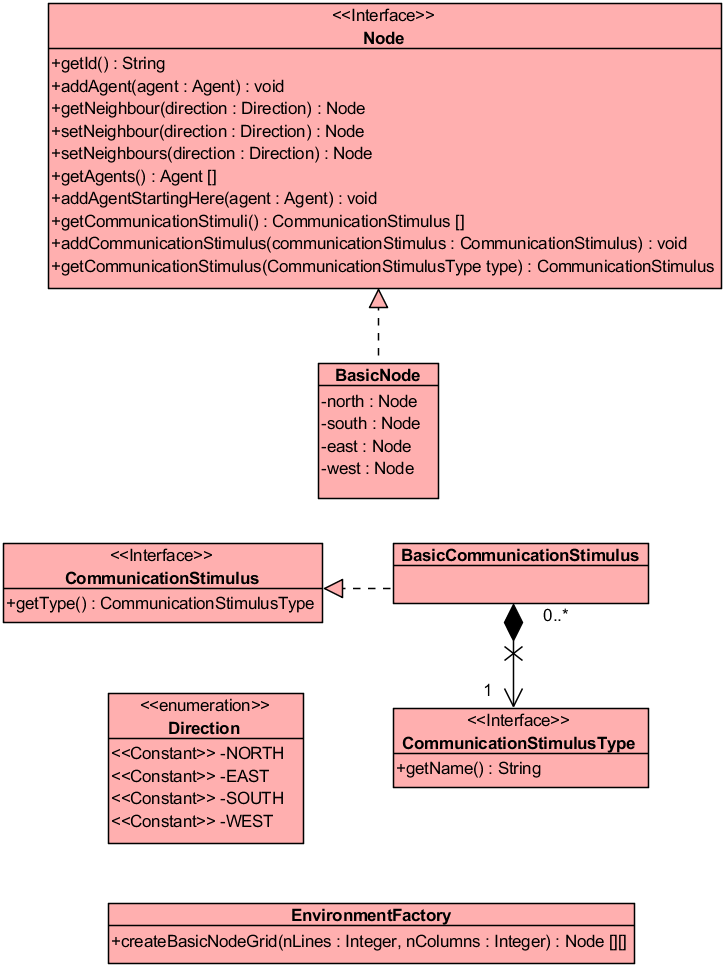
\includegraphics[width=1.0\linewidth]{gfx/uml-env-package.png}
  \caption{Generic model of environment package}
  \label{fig:gen-env-package}
\end{figure}

\section {Agents}
\label{sec:agents}

To enable the agents defined by the model to enjoy the properties that define agents in general it is critical that they have their own lifecycle, and the most flexible way to achieve that is if each agent is run in an isolated thread in one of the available CPUs of the machine running the simulation. This is guaranteed by the \emph{AbstractAgent} which implements the \emph{Callable} interface (see section \ref{subsec:threads-task-exec} for more details).  

The abstraction of any agent is the \emph{Agent} interface though. It formalises the basic API that is available to any agent in the model. The most relevant are:

\begin{itemize}
  \item String getId(): Each agent must have an unique identifier string to be used for identification. This method returns it. Note that is up to the user to make sure this string is unique.
  
  \item AgentType getAgentType(): Returns the type associated with the agent.
  
  \item void setCurrentNode(Node): Places the agent in a specific node of the environment.
\end{itemize}

There are another methods that are related with tracking the nodes the agent has been in the environment during the simulation, more information on these methods can be found in the appendix \ref{chapter:model-code}.

The \emph{AbstractAgent} is the base abstract implementation of the \emph{Agent} interface. It implements all the public methods declared by the interface, plus declares the implementation of the \emph{Callable} interface, returning the type \emph{Void}, which is a convention to tell the compiler that no value is expected to be returned. By being abstract and declaring the implementation of \emph{Callable}, the class effectively forces any concrete specialisation class to implement the methods that define a task in Java, therefore allowing any agent to be executed in an isolated thread.

\subsection{Task Agents}

The smallest unit of work in the computational model is a task, and they are the means to agents to get things done. Please note that this task is different from a Java task discussed in section \ref{subsec:threads-task-exec}. 

In order to enable agents to execute tasks the concrete specialisation of the \emph{AbstractAgent} class, the \emph{TaskAgent} class has a synchronised field called \emph{currentTask} that contains a reference to the task that the agent is executing at the moment. The second difference from the super class, is that task agents have a different \emph{type} associated to them, a \emph{TaskAgentType}, this is important because it is in the \emph{TaskAgentType} that the tasks that an agent is capable of executing are defined, see section \ref{sec:taskagentype} for more details.

\subsection{Agent Types}
\label{sec:agent-types}

In nature individuals use different ways to differentiate themselves from other individuals, in the proposed computational model each agent belongs to a specific type, something that define them as a class. The \emph{AgentType} interface formalises the most basic abstraction of a type of agents.  It has only one method:
\begin{itemize}
  \item String getName(): Returns the name of that type, must be unique.
\end{itemize}
As in the previous cases, the interface does not have any mechanism to make sure a type has a unique name, it is up to de user to make sure that is the case.

An implementation of \emph{AgentType} provides the means for agents to distinguish themselves if necessary, one agent can check another agent’s type when they are in the same node, this is very important, because one agent can react differently if it comes across another agent of the same type or if it encounters an agent that might impose some sort of danger.

In the sake of performance, agent types must implement the Singleton Pattern, which guarantees only one object instance of a type only.\cite{bloch2008effective} If agent types were not to be singletons, every time a new agent is instanced a new agent type and the other objects that compose it, like tasks, are going to be created as well, consuming large amounts of memory. 

\subsubsection{The TaskAgentType type}
\label{sec:taskagentype}

The \emph{TaskAgent} interface is simple and has only one method:

\begin{itemize}
  \item List<Task> getTasks(): Returns a list of tasks that the agents of this type are able to execute.
\end{itemize}

The enumeration \emph{BasicTaskAgentType} is a reference implementation of the interface. Agents of that type are able to execute only one task, \emph{WandererTask}, see section \ref{sec:wanderer-task} for more details on the task.

\subsection{The Ant Interface}

The ant implementation of the model starts from the \emph{Ant} interface. It declares the public API for any agent that is an ant. The most relevant methods are: 

\begin{itemize}
  \item Direction getMovingDirection(): Returns what direction the ant is moving in relation to the environment grid.
  \item void incrementStimulusIntensity(ChemicalStimulusType): Lay pheromone onto the current node that the agent is at.
  \item double collectFood(Agent, double): Tries to collect the specified amount of food from the food source specified as parameter, returns the amount of food that the agent was able to collect.
  \item Boolean isCaringFood(): Returns true if the agent is caring food, false otherwise.
  \item FoodSourceAgent findFoodSource(): Checks if any agent in the current node is a food source, if any is found it is returned otherwise \emph{null} is returned.
  \item void invertDirection(): Inverts the direction the agent is traveling, for example, if the agent is traveling East, after this method is called the agent’s moving direction will be West. See section XXX for more details.
  \item void depositFood(AntNestAgent): Deposit the food the agent is caring into the nest passed as parameter.
\end{itemize}

For the full API and more detail explanations of all the methods, please see section XXX.

\subsection{Ant Agents}

The \emph{AntAgent} class offer an implementation of the \emph{Ant} interface. Mostly important it has three private methods that are used by \emph{incrementStimulusIntensity (ChemicalCommStimulusType)} for laying pheromone onto the environment. As seen on section \ref{subsec:chemical-stimulus} chemical communication stimulus types have a propriety called \emph{radius} that defines the reach of that particular stimulus around the node where it was deposited, these three methods use this information when depositing pheromone. The intensity of the stimulus decreases as the distance from the node where the agent is at increases according to the following: 

\begin{equation}
intensity_{new} =  intensity_{current} + increase * (1 / distance)
\end{equation}

Figure \ref{fig:distanse-vs-inc} shows how the intensity of the deposited amount of chemical stimulus varies according to the distance to the node the agent is executing the increment. The amount of stimulus that each agent increments is defined by the agent type, see section \ref{sec:agent-types} for a detailed explanation.

\begin{figure}[H]
  \centering
  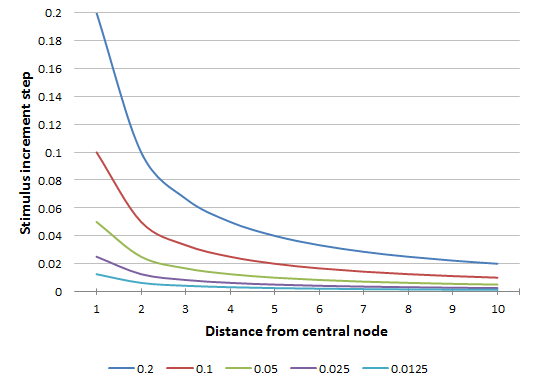
\includegraphics[width=0.5\linewidth]{gfx/distance-vs-increment.png}
  \caption{Variation of increment according to distance to central node}
  \label{fig:distanse-vs-inc}
\end{figure}

Figure \ref{fig:intensity-example} illustrates how the pheromone is laid depending on the radius of the stimulus. The strong the increment is the brighter the red. Each node is represented by a single square. In the image three different radius are demonstrated, form left to right we have 2, 4 and 5 respectively. It is clear that he increment falls as the distance from the central node gets bigger.

\begin{figure}[H]
  \centering
  
\includegraphics[width=0.5\linewidth]{gfx/intensity-example.png}
  \caption{Pheromone deposit for stimulus with different radius sizes}
  \label{fig:intensity-example}
\end{figure}

\subsection{Ant types}

The interface \emph{AntType} and its implementations are used to represent any specific type of ant in the computational model. The interface declares the following methods:

\begin{itemize}

  \item void execute(Agent): Method executed when the agent is executed by the thread pool.
  \item double getStimulusIncrement(String): Returns the amount of stimulus the agent is able to lay.
  \item int getMemorySize(): The number nodes the agent can remember it has been.
  \item double getAmountOfFoodCapableToCollect(): Returns the amount of food the agent is capable of caring 

\end{itemize}

(((need to discuss the way the memory is implemented)))

By far the most important method in the list is \emph{void execute(Agent)}, because this method is the method that defines the agent's behaviour. It is in this method the agent can analyse the environment state around it and decide which tasks to execute.

As seen, different type of ants are able to deposit different types of pheromone and in different quantities. So every type of ant has a map that tells by name, what is the increment for each stimulus the ant is able to deposit. the method \emph{double getStimulusIncrement(String)} is used to query these amounts.

\subsubsection{WorkerType}

The enumeration \emph{WorkerType} defines the type of ant that represent workers in a colony. The type is capable of executing three tasks, \emph{ForageTask}, \emph{FindHomeTask} and \emph{FindAndHideInNestTask}. Ants of this type are sensitive can lay \emph{ForageStimulusType} and low quantities of \emph{WarningStimulusType}. 

The goal of this type of ant is to explore the environment, find food,  collect as much as possible and take it back to the nest. Figure \ref{fig:worker-type} fully describes the algorithm implemented by the \emph{WorkerType}.

\begin{figure}[H]
  \centering
  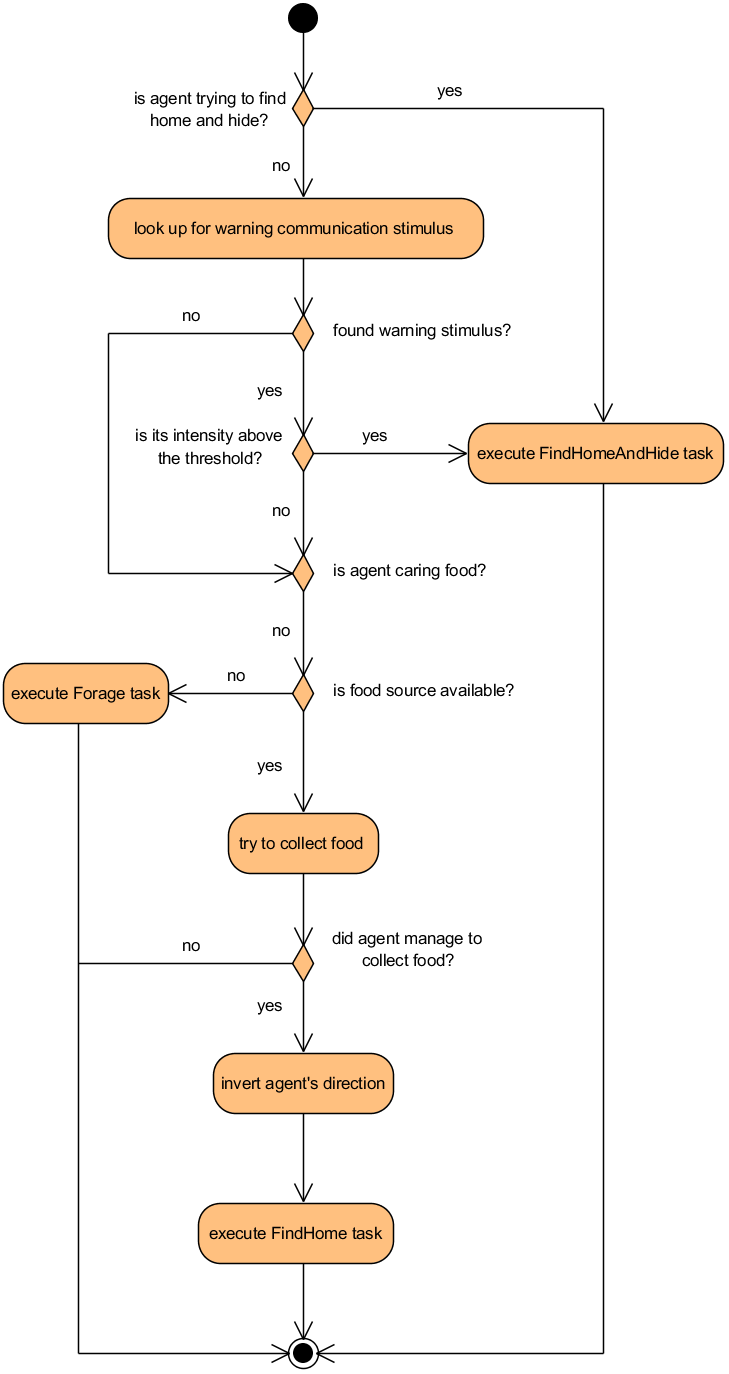
\includegraphics[width=0.8\linewidth]{gfx/uml-worker-type.png}
  \caption{Worker Type ant algorithm}
  \label{fig:worker-type}
\end{figure}

\subsubsection{Ant Nests}

The enumeration \emph{AntNestType} declares a type of agent that represents an ant nest. It implements the base \emph{AgentType} interface, so as one would expect, agents of this types are not able to execute tasks.

The class \emph{AntNestAgent} is an specialisation of \emph{AbstractAgent}, it has an extra synchronised field that works as a counter of how much food is available in the nest, \emph{amountOfFoodHeld}. It also declares a public method called \emph{void addPortionOfFood(AntAgent, double)} which allows ants to deposit food in the nest.

\subsection{Agents Package}

\begin{figure}[H]
  \centering
  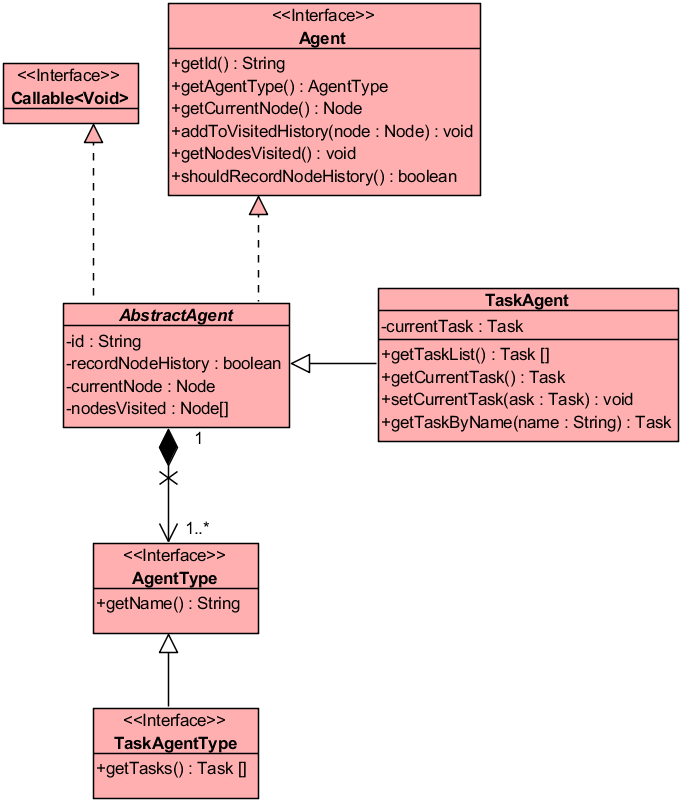
\includegraphics[width=1.0\linewidth]{gfx/uml-agent-package.png}
  \caption{Generic model of the agent package}
  \label{fig:gen-agent-package}
\end{figure}


\section {Tasks}

Tasks are a unit of specialised work. They are the means to agents to do something they need to do. Different type of agents can share the same task, but it is up to each of them how to use it.

The \emph{Task} interface formalises two methods:

\begin{itemize}
  \item String getName(): Returns the unique name that identifies the task.
  
  \item void execute(Agent): Runs the task algorithm for the agent used as parameter.
\end{itemize}

Tasks are a convenient way to process unit of work that are isolated one from another and done by more than one type of agent. The \emph{void execute(Agent)} method contains the actions that the task is to perform, the agent that is requesting the task execution is passed as a parameter so the task is able to access the agent's context, such as neighbours and communication stimuli. The \emph{AbstractTask} class provides the base implementation for concrete tasks.

\subsection{Wanderer Task}
\label{sec:wanderer-task}

This task is a simple task that agents can use when they are exploring the environment, it causes the agent to move from the current node to one of the available neighbours. It selects which neighbour to move to completely at random.

In the case of ants, for example, they use this task when looking for a new source of food or when they reach one of the environment boundaries and need to switch their moving direction.

\subsection{Ant Tasks}
\label{sec:ant-tasks}

Ants execute tasks that implement the \emph{AntTask} interface. For the list of methods of the interface, please see XXX.

\subsubsection{Forage Task}
\label{task:forage}

The \emph{ForageTask} is also used by agents to find food sources and collect food. Differently from the \emph{WandererTask}, it does not pick a node to move to at random, it follows the forage chemical stimulus trail.

Although the pheromone trail is the most important part when the agents are deciding where to go next, another effects should be considered, for instance an agent could be taken away from the trail by the wind or if some information, like chemical landmarks, that the ants use to locate themselves is modified, should somehow be considered. Tt virtually impossible to model all this cases though, more, it would be wrong to try to model all the possible interferences in the colony.

So, the agents present a stochastic behaviour as far as moving through the space is concerned. So the process of choosing the node to move to consists of: 

\begin{enumerate}
  \item Each neighbour node is associated with a weight.
  \item The weights are multiplied by the actual pheromone trail found in  each of the neighbour nodes.
  \item The results of each multiplication in the previous step are summed up to a total.
  \item Each multiplication of step 2 is divided by the total, in order to find their ratio.
  \item A Monte Carlo (((cite))) like selection on the neighbour nodes is executed using these rates.
\end{enumerate}

\begin{figure}[H]
  \centering
  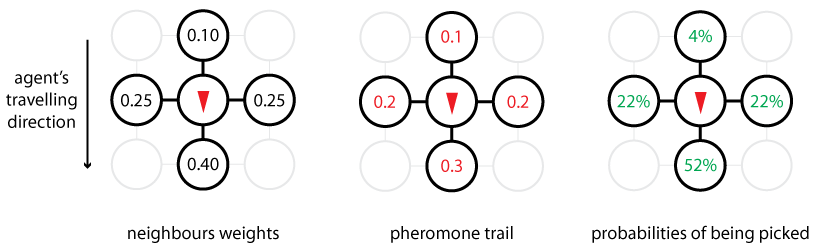
\includegraphics[width=0.9\linewidth]{gfx/choosing-next-node.png}
  \caption{Elements used to select next node to move to}
  \label{fig:choosing-next-node}
\end{figure}

Figure \ref{fig:choosing-next-node} illustrates these steps. It is important to understand that when applying the weights to the neighbours the task uses the agent as reference not the grid. As an example, if we imagine a agent with the moving direction set to East in relation to the grid, so the east neighbour from the node that the agent sits is pointing to the north direction of the agent. Figure \ref{fig:position-reference} illustrates that.

\begin{figure}[H]
  \centering
  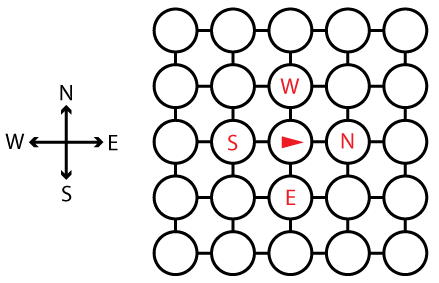
\includegraphics[width=0.5\linewidth]{gfx/reference.png}
  \caption{Reference of directions}
  \label{fig:position-reference}
\end{figure}

It is necessary to know what direction the agent is travelling to and perform this transformation between the grid direction reference to the agent's in order to apply the right selection weights to the neighbour nodes.

This method of selection is implemented by the utility class \emph{AntTaskUtil} and is used in other tasks as well. The method is flexible enough to allow tasks to set their own weights for the neighbour nodes and ask any type of chemical stimulus to be used in the calculation.

Figure \ref{fig:forage-activity} is the active diagram of the algorithm implemented by the \emph{void execute(Agent)} method of the \emph{ForageTask}.

\begin{figure}[H]
  \centering
  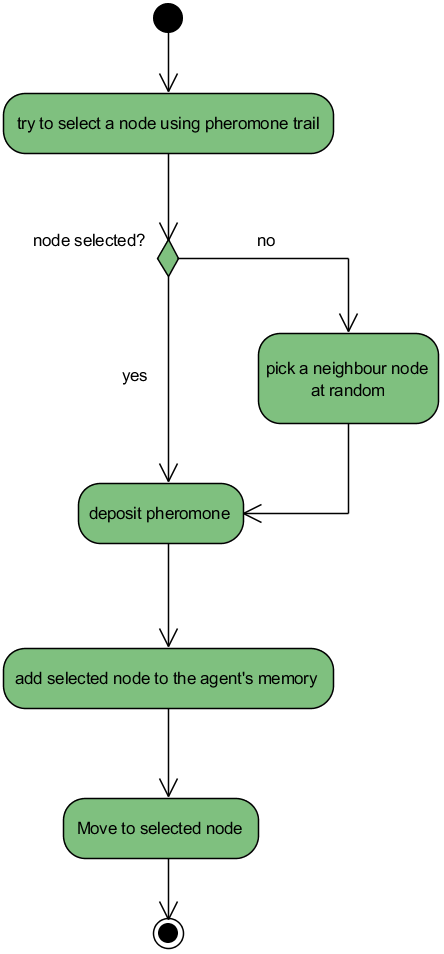
\includegraphics[width=0.6\linewidth]{gfx/uml-act-forage.png}
  \caption{Forage task execution activity diagram}
  \label{fig:forage-activity}
\end{figure}

\subsubsection{Find Home Task}
\label{task:find-home}

The \emph{FindHomeTask} is useful for ants that have collected food and need to deposit it in their nest. It uses the same procedure that \emph{ForageTask} to select which node to move next. The biggest difference is that it tries to use the agent's memory before following the specified pheromone trail. The task's algorithm is illustrated in Figure \ref{fig:find-home-act}.

\begin{figure}[H]
  \centering
  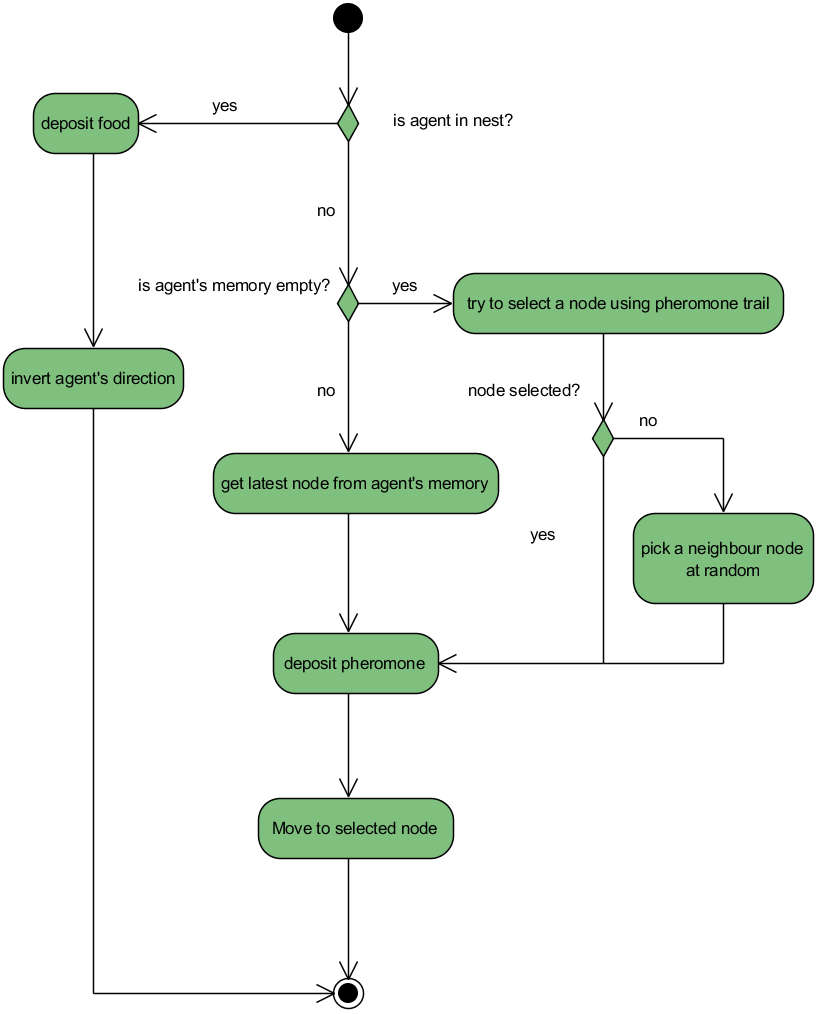
\includegraphics[width=0.9\linewidth]{gfx/uml-act-home.png}
  \caption{Find home task execution activity diagram}
  \label{fig:find-home-act}
\end{figure}

\subsubsection{Find Home And Hide}
\label{task:find-home-hide}

The \emph{FindHomeAndHideTask} is very similar to \emph{FindHomeTask} the only difference is that if the agent is in a node that contains a nest the task does not try to do anything else, it leaves the agent there. 

is useful for ants that have collected food and need to deposit it in their nest. It uses the same procedure that \emph{ForageTask} to select which node to move next. The biggest difference is that it tries to use the agent's memory before following the specified pheromone trail. The task's algorithm is illustrated in Figure \ref{fig:find-home-hide-act}.

\begin{figure}[H]
  \centering
  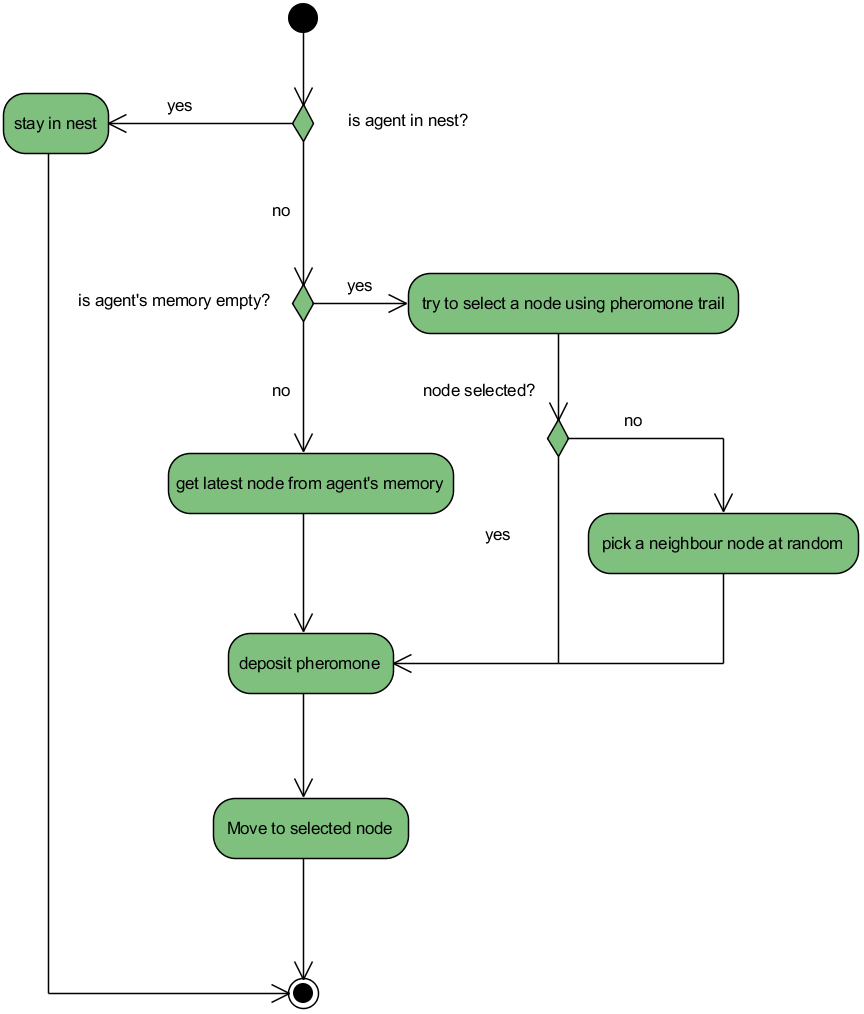
\includegraphics[width=0.8\linewidth]{gfx/uml-act-home-hide.png}
  \caption{Find home and hide task execution activity diagram}
  \label{fig:find-home-hide-act}
\end{figure}

\section {Generic Computational Model Diagram}

\begin{figure}[H]
  \centering
  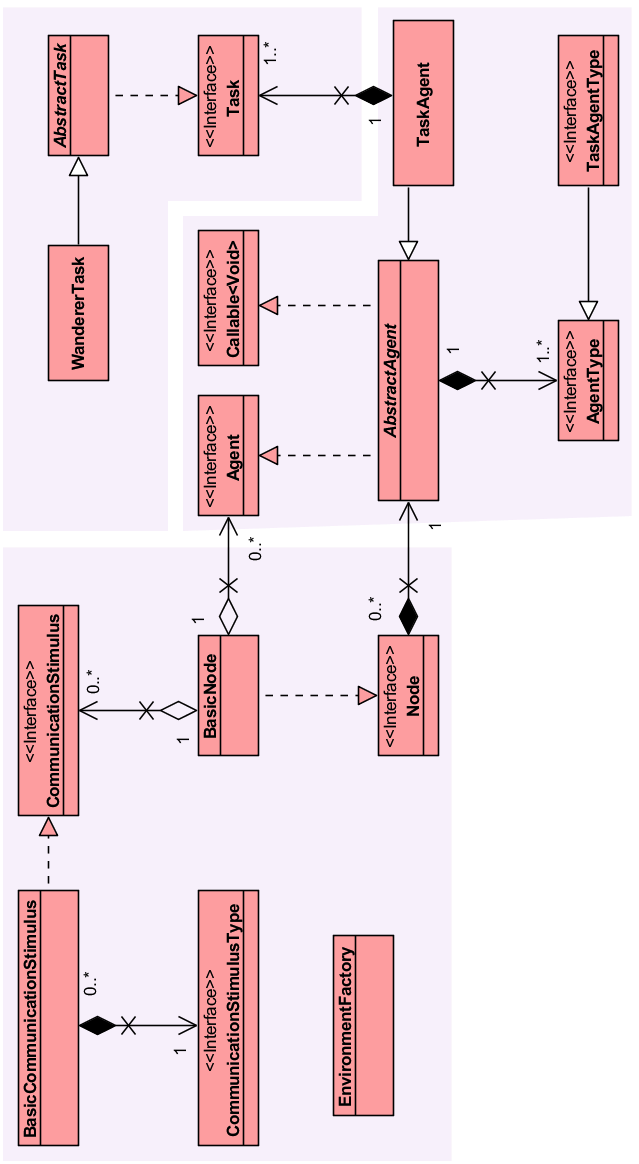
\includegraphics[width=0.7\linewidth]{gfx/uml-generic-overview.png}
  \caption{Generic Computational Model}
  \label{fig:generic-model}
\end{figure}